Already in the year 2010 the user \textit{ByteCoin} described the idea of selfish mining in the Bitcoin forum \textit{bitcointalk} \cite{ByteCoin2010}.
He provided simulation results of the attack which at that time was called \textit{mining cartel attack}.
Nevertheless, the discussions in the thread never caught fire and no further investigations or countermeasures were taken by the community \cite{BitcoinTalk2010, bahack2013theoretical}.

Later in 2014 \cite{eyal2014majority} released the paper \textit{"Majority is not enough: Bitcoin mining is vulnerable."} and coined the term selfish mining.
The paper gives a formal description of selfish mining and proves how a miner can earn more than his fair share by conducting the attack.
Figure \ref{fig:selfish_mining} shows the attack as a state machine where $\alpha$ denotes the mining power share of the selfish miner.
The labels of the states are representing the lead of the selfish miner over the public chain.
Whenever the public network finds a block and the selfish miner publishes a competing block of the same height a block race occurs denoted with the state \textit{0'}.
In the case of such a block race, the variable $\gamma$ expresses the probability of the selfish miner to win the block race.
Hence $\gamma$ part of the miners are mining on the public-private block and respectively $(1 - \gamma)$ are mining on the public block.
The labels on the transitions are representing the transition probabilities between the states.
The profitability of the simple strategy of \cite{eyal2014majority} was proven by using probability calculations based on the state machine of figure \ref{fig:selfish_mining}.
Furthermore, results of an undisclosed Bitcoin protocol simulator were given.
In the simulation, 1000 miners with the same mining power were simulated and a fraction of these miners formed a pool which applied the selfish mining algorithm.
In the case of a block race they artificially split the network where one part is mining on the public block and one part is mining on the block of the selfish pool.

\begin{figure}[t]
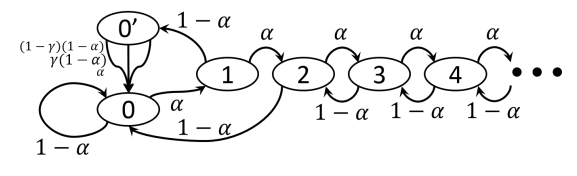
\includegraphics[width=8cm]{selfish_mining}
\centering
\caption{Selfish mining state machine with transition probabilities \cite{eyal2014majority}}
\label{fig:selfish_mining}
\end{figure}


Further research showed that more generalised selfish mining strategies lead to even more relative gain for the selfish miner \cite{nayak2016stubborn,sapirshtein2016optimal, gervais2015tampering, gervais2016security, bahack2013theoretical}.
Figure \ref{fig:stubborn_mining} shows a possible categorization of the different selfish mining strategies where $\alpha$ and $\gamma$ is used equivalent as in figure \ref{fig:selfish_mining} and $\beta$ expresses (1 - $\alpha$).
Furthermore, the prime states are standing for states where a block race happens on certain height and the \textit{0''} represent the state where both chains have the same height but the selfish miner and the rest of the network are mining on different branches.
The idea behind the different variations of selfish mining strategies in figure \ref{fig:stubborn_mining} are:
\begin{itemize}
\item Lead stubborn mining strategy compromises the idea to cause as many block races as possible and to never overwrite the public chain with a longer chain.
This strategy continuously tries to split the network to mine on different blocks and is therefore especially promising when the probability to win the block race is very high.
\item Equal-fork stubborn mining strategy changes the selfish mining strategy just by one transition.
In case the selfish miner finds a block during a block race, he does not publish his block to win the race but he also keeps this block undisclosed to secretly mine on this new tip of the chain.
\item Trail stubborn mining strategies reflects the idea to even trail behind the public chain and to eventually catch up.
The figure \ref{fig:stubborn_mining} depicts the trail stubborn mining strategy \textit{T1}.
The number one denotes that the selfish miner is allowed to trail one block behind the public chain.
\end{itemize}

The strategy space for a selfish miner is practically endless and combinations of the aforementioned strategies are possible and are leading to even more relative gain compared to honest miners\cite{nayak2016stubborn,sapirshtein2016optimal, gervais2015tampering, gervais2016security, bahack2013theoretical}.


\begin{figure}[t]
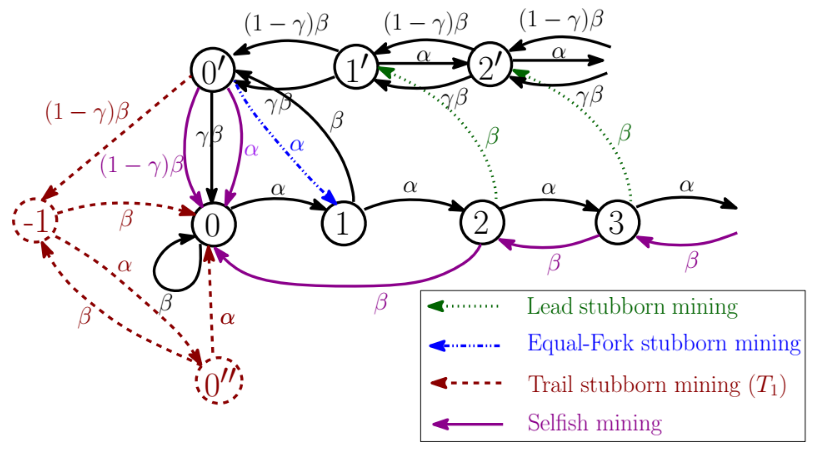
\includegraphics[width=10cm]{stubborn_mining}
\centering
\caption{Categorization of different mining strategies \cite{nayak2016stubborn}}
\label{fig:stubborn_mining}
\end{figure}


To find the best strategy for a given mining power share $\alpha$ and connectivity $\gamma$ researchers used different methodologies.
\cite{gervais2015tampering, nayak2016stubborn} used numeric simulations of paths in the state machine to find optimal selfish mining strategies.
\cite{sapirshtein2016optimal, gervais2016security} on the other hand used MDPs based on a state machine to find strategies with the most relative gain.
The basic structure of the used state machines is for all publications the same.
To further validate their results \cite{eyal2014majority, sapirshtein2016optimal} used a closed-source simulation.

Besides using variations of the selfish mining strategies, the attack can also be combined with other attacks to achieve better results \cite{gervais2016security, sapirshtein2016optimal, nayak2016stubborn, gervais2015tampering}.
If the eclipse attack is used in combination with selfish mining the victim contributes its mining power to the private chain and hence, strengthens the position of the selfish miner \cite{nayak2016stubborn, gervais2016security}.
\cite{nayak2016stubborn} additionally shows that the eclipsed victim under certain circumstances can benefit from the attack and therefore has no incentive to stop the attack.
Another attack which can be used in combination with selfish mining is double-spending \cite{sapirshtein2016optimal, gervais2016security}.
Every time the selfish miner starts his selfish mining attack he can publish a transaction and include a conflicting transaction in his first secret block.
During the execution of the selfish mining attack, the payment receiver may accept the payment depending on his block confirmation time.
Now in the case of a successful selfish mining attempt, the adversary can overwrite the public chain, which additionally results in a successful double spending.
The operational costs of unsuccessful double-spending can be seen as low because the adversary still would get goods or a service in exchange for the transaction \cite{sapirshtein2016optimal, gervais2016security}.

Last but not least also the prevention of selfish mining is part of the current work in selfish mining research \cite{eyal2014majority, billah2015one, solat2016zeroblock, zhang2017publish}.
A backwards-compatible patch to mitigate selfish mining is uniform tie-breaking \cite{eyal2014majority}.
This means whenever a node receives two blocks of the same height he randomly select on of the blocks to mine on.
\cite{eyal2014majority} showed that this would raise the profit threshold to 25\% of the computational power and hence mitigating selfish mining.
The drawback of this proposed change is that it would increase the connectivity of badly connected attackers to almost 50\% with no actual effort for them.
Ethereum, the currently second largest cryptocurrency by market capitalization \cite{marketcap2017}, has implemented uniform tie-breaking as a countermeasure against selfish mining \cite{gervais2016security, unifromtiebreakingethereum}.
Another countermeasure foresees unforgeable timestamps to secure Bitcoin against selfish mining \cite{billah2015one}.
This countermeasure would make all pre-mined blocks of the selfish miner invalid after a certain amount of time.
The implementation of this patch would require random beacons and hence introduce complexity and a new attack vector \cite{billah2015one}.
\cite{zhang2017publish} proposes backward-compatible countermeasure by neglecting blocks that are not published in time and allows incorporation of competing blocks in the chain similar to Ethereum's uncle blocks \cite{wood2014ethereum}.
This enables a new fork-resolving policy where a block always contributes to neither or both branches of the fork \cite{zhang2017publish}.
All of this mentioned countermeasures are not planned to be implemented or implemented in Bitcoin \cite{bitcoin, bitcoinbip}.
